%\documentclass[11pt]{amsart}
\documentclass[review]{siamart}
\usepackage{geometry}                % See geometry.pdf to learn the layout options. There are lots.
\geometry{letterpaper}                   % ... or a4paper or a5paper or ... 
%\geometry{landscape}                % Activate for for rotated page geometry
%\usepackage[parfill]{parskip}    % Activate to begin paragraphs with an empty line rather than an indent
\usepackage{graphicx}
\usepackage{amssymb}
\usepackage{epstopdf}
\DeclareGraphicsRule{.tif}{png}{.png}{`convert #1 `dirname #1`/`basename #1 .tif`.png}
\newcommand{\Order}[1]{\ensuremath{\mathcal{O}(#1)}}    % big O notation


\title{Algorithms and software for extreme-scale particle-in-cell simulations of highly magnetized plasmas}
\author{Mark F. Adams\and Tobin Issac\and Mathew Knepley}
\nolinenumbers
\begin{document}
\maketitle

Efficient, engineering relevant, simulations of highly magnetized fusion plasmas is one of the great computational science challenges of today.
The governing equations, the Boltzmann-Maxwell system, are a set of 6D nonlinear hyperbolic equations with dynamics coupled over many decades of time and length scales.
The high dimensionality of these problems lend themselves to particle-in-cell (PIC) methods.
Additionally, the strong, complex guide fields of tokamaks generate highly anisotropic models that pose significant challenges to accurate and efficient discretizations and solvers.
Simulating highly magnetized fusion plasmas for ITER, with the accuracy and reliability necessary to be relevant to it's design and operation, is an important challenge for one of the largest scientific experiments of today, ITER.
We propose to contribution to this effort by developing efficient methods for PIC simulations in general, and for fusion plasmas in particular, and by deploying implementations, optimized for emerging architectures, in the PETSc numerical library \cite{KnepleyBrownMcInnesSmithRuppAdams2015b}, for use by the computational plasma physics community.

\section{Introduction}

The high degree of concurrency of emerging architectures at extreme-scale, and the high relative cost of data movement, requires careful data placement to efficiently utilize computational resources.
The importance of data locality is not new, the pressures on memory systems have been building for decades, because floating point processing speeds increase faster than data movement speeds, but the massive concurrency of emerging architectures is further exacerbating the need for careful data layout in extreme-scale computing.
This is a challenge for PIC codes because they process data in two very different data structures, which interact in particle-cell kernels such as charge deposition to the grid and particle gradient computation from the grid.
Additionally, optimal data decompositions of different computational components can be very different.
For instance, the collision operator and the deposit, solve, push phase have inherently different natural data partitionings, and a ``transpose" to move particle between these partitions has a cost.
Balancing this cost with the rest of the computation is a common tradeoff in computational science and can be seen in, for instance, the Eulerian fusion plasma code Gysela \cite{Bigot13}.

The PETSc community has extensive experience in extreme-scale solution methods for PDEs (discretizations, meshing,  nonlinear solvers, time integrators, optimization solvers, etc.) and in the deployment of optimized implementations of these methods to the public.
Fast solvers also require careful data placement for optimal performance, but PIC methods add new sets of constraints and opportunities for optimizing algorithms for extreme-scale emerging architectures.
To this end, we focus on grid management to support the development of optimal data decomposition and algorithms, or data models,  for the efficient processing of particle-cell interactions, as well as fast solvers for, for example, Poisson's equation, Ampere's law, and the magnetohydrodymaic  solvers of implicit PIC methods \cite{DBLP:journals/cphysics/ChenC15}.

This document describes the support for extreme-scale PIC simulations on emerging architectures under development in PETSc.
We build on the Solver Integrated Tree-based Adaptive Refinement (SITAR) infrastructure in PETSc, for fast and accurate PDE discretizations, meshing, and solvers.
We extend SITAR with methods and features to support the development of efficient and scalable data models and algorithms for engineering relevant simulations of fusion plasmas by the computational plasma physics community.
In addition to this PETSc library work, this document describes a tokamak PIC code, X2 (\S\ref{sec:x2}).
X2 is designed from the ground up for extreme scalability and extensibility to emerging architectures.
X2 is used to drive the library development and explore the algorithmic space of modern extreme scale PIC methods, and to provide data on the potential usefulness of these PETSc resources for PIC applications.

\section{Background}

PIC methods are popular for discretizing high dimensional problems in a variety of fields because of their low cost relative to full grid or Eulerian methods on such problems, although Eulerian methods are often at least hybridized with PIC in, for instance, the collision operator.
PIC methods do have disadvantages, including more complex data algorithms because of its two distinct data types, particles and cells.
PIC algorithms require three types of processing: 1) particle processing (e.g., the evolution of Vlasov's equation), 2) grid processing (e.g., solvers), and 3) particle-grid interactions (e.g., particle charge deposition and gradients of potentials for particle pushing).
Pure particle processing, such as the ``push" of particles use relatively simple arrays and each particle can be processed concurrently.
Most, say well over $99\%$, of the data in a fusion PIC simulation is in the particles.
Thus, pure grid work, such as the Poisson solver, have abundant computational resources available and, for instance, can be run entirely on the CPU of accelerated architectures, or on a reduced set of cores on symmetric systems.
Particle-grid interactions are challenging because the data structures and natural data decompositions are different, but are tightly coupled algorithmically.
This tight coupling, and the ever increasing importance of data locality generally, make the data model critical in the current and future extreme-scale PIC applications.

The critical importance of data placement for the efficient processing of PIC methods requires that highly optimal, and potentially complex, data models be developed.
The fusion PIC community has avoided much of this complexity by replicating all grid data on each MPI process or address space.
This approach does of course solve this problem of data layout by simply replicating it everywhere, but it also removes a powerful design space of algorithms to optimize extreme-scale PIC codes.
Distributing grids will be very disruptive to the code base of fusion PIC applications, but many future optimization in the context of this obsolete data model will not be applicable, or necessary, on distributed grids.
 It behooves the fusion PIC community to move to distributed data models as soon as possible.

The physics community has developed a large body of research and experience in using PIC methods for fusion plasmas and they are one of the largest users in DOE leadership class compute facilities.
The applied math, engineering, and physics communities have developed powerful discretization and solver methods for extreme-scale computing in just the past ten years and stretching back to the 1960s, but these modern methods are not widely used in the fusion PIC community.
The continued advancement of computational fusion physics within DOE, and the global community, especially as we move from only verifying computational results with theory to reliable predictive analysis, requires that both modern numerical methods and parallel computing techniques, as well as reliable software engineering methodologies, be employed.

The engineering complexity required to develop a flexible infrastructure that allows for the expression of the most optimal algorithms demands a higher level of software quality assurance processes than is often present in the codes that are driven by academic reward systems, such as number of journal publications, as opposed to the demands for reliable predictive analysis that drives the commercial sector.
Commercial grad software engineering takes both skill and time that is not available to most academic physics code projects and is not seen as worth to cost due to their academic reward structure.
PETSc employs commercial grade software engineering processes and some of our users, even those that work in academia, follow our practices because in the long term it leads to higher productivity even by the standards of their academic field. 
This project provides fusion PIC codes with solid infrastructure on which to build their physics, to allow for the full use of their theoretical expertise without the demands of implementing, verifying, and maintaining the ever increasing software stack required to effectively use modern hardware.

This work amortizes both the development costs and the intellectual resources required to develop and deploy support for extreme-scale PIC applications.
This work builds on the SITAR framework in PETSc, which provides both fast solvers, tightly integrated meshing and discretizations, and optimized implementation for emerging architectures \cite{KnepleyBrownMcInnesSmithRuppAdams2015}.
SITAR is built on the highly scalable algorithms and implementations in the p4est distributed tree library \cite{DBLP:journals/siamsc/IsaacBWG15,Rudi:2015:EIS:2807591.2807675,Stadler1033}.

\section{Methodology}

The methods developed in this project are guided by several general principles in terms of algorithms pursued in X2 and supported in PETSc.
These principles reflect our evolving view of algorithms for extreme-scale fusion PIC methods and desire to deploy an complete, if simple, early version of these methods so that we can begin to experiment in the design space of these algorithms and provide an early avenue for physics colleagues to contribute physics features (e.g., gyrokinetics).
Our methodology has the following desired features:
\begin{itemize}
\item flexible local grids to allow for particle-grid interaction with non-local parts of the grid;
\item hierarchical grids for fast geometric multigrid solvers, adaptive mesh refinement (AMR), and the ``particle search" method to determine the address space of a particle;
\item grids abstracted from application scientists to allow multiple types of grids and discretizations to be supported and selected at run time;
\item fast linear and nonlinear solvers for Poisson and Ampere's law solvers, and implicit PIC methods (magnetohydrodymaic);
\item incremental problem development for debugging and verification on Cartesian grids and ramping up to full tokamak wall geometries;
\item finite particle form factors, or density smoothing, to allow for arbitrary mesh resolution without increasing particle count to avoid particle noise;
\begin{itemize}
\item allows decoupling grid spacing from particle form factor and facilitates AMR and convergence test verification;
\end{itemize}
\item finite volume (FV), discontinuous Galerkin(DG), and finite element (FE) discretizations;
\begin{itemize}
\item conservative discretizations (FV and DG) are useful for flux surface averaging projections although we are beginning with FE;
\end{itemize}
\item architecture specific computational kernels for emerging architectures \cite{KnepleyBrownMcInnesSmithRuppAdams2015};
\item incremental contributions to the plasma physics community (\S\ref{sec:id}).
\end{itemize}

\subsection{Incremental Development}
\label{sec:id}

The realization of an engineering relevant full plasma simulation of ITER is a significant multi-year undertaking.
The development plans for this project are to be both incrementally relevant and engaged with the physics community.
To this end, early deliverables are important, to encourage physicists to participate with us and for us to stay grounded in the real engineering demands.
To this end we see several early areas that our project can contribute:
\begin{itemize}
\item Distributed data model exploration. Explore data decompositions and collect performance data to help further refine effective distributed data models for fusion PIC applications;
\item Code verification. Cross code verification of existing fusion PIC codes, on somewhat simple model problems, but with full ITER wall geometries;
\item Performance Verification.  Develop performance models of idioms in PIC codes (e.g., equation solvers, particle communications, particle pushing) to help application scientist verify that codes are performing correctly, by understanding the relative costs of different processes and their sensitivities (derivatives with respect to) machine metrics.
\end{itemize}
 

\section{Current Development}
\label{sec:x2}

The development proposed herein takes place in a branch in the PETSc repository (mark/feature-picell) and a driver application named X2 (DMPICell ex1.c).
Code will likely migrate from X2 into the PETSc library as development progresses.
X2 is intended to be used to gather initial performance data on modern architectures to guide further data model developments, and to verify the PETSc library code.
Our approach is to exploit the fact that particle distributions, at least from a computational point of view, are relatively uniformly distributed over the domain and our grids are quasi-uniform.
This allows for particle distributions that are simply attached to cells of the solver grid, but load is balanced by using a weighted cell partitioning.

We currently use guide center particles only (i.e., only a parallel velocity, resulting in a 4D method), which simplifies charge deposition.
These two simplifications allow us to reuse particle infrastructure that has been developed for other PETSc PIC users \cite{may2014ptatin} that attach particle to solver cells in the particle push kernel.
More complex data models with extended halo regions to accommodate gyrokinetic methods (finite shape) and high order (explicit) time integrators will be likely developments in the future.

The collision operator is a computational intensive nonlinear solve in velocity space on each particle collision cell.
Flux tubes are a natural choice for these collision cells, these are long, narrow subdomains that follow the twisting magnetic field lines around the torus.
We decouple the grid partitioning from the flux tube partitioning and implement a full ``transpose" of particles between these two partitions.
Aligning the solver partitioning with flux tubes, to minimize communication, is a potential future optimization.

Figure \ref{fig:cross} (left) shows an example of four flux tubes on a half torus and Figure \ref{fig:cross} (right) shows an example of half a coarse grid of ITER.
\begin{figure}[h!]
   \centering
   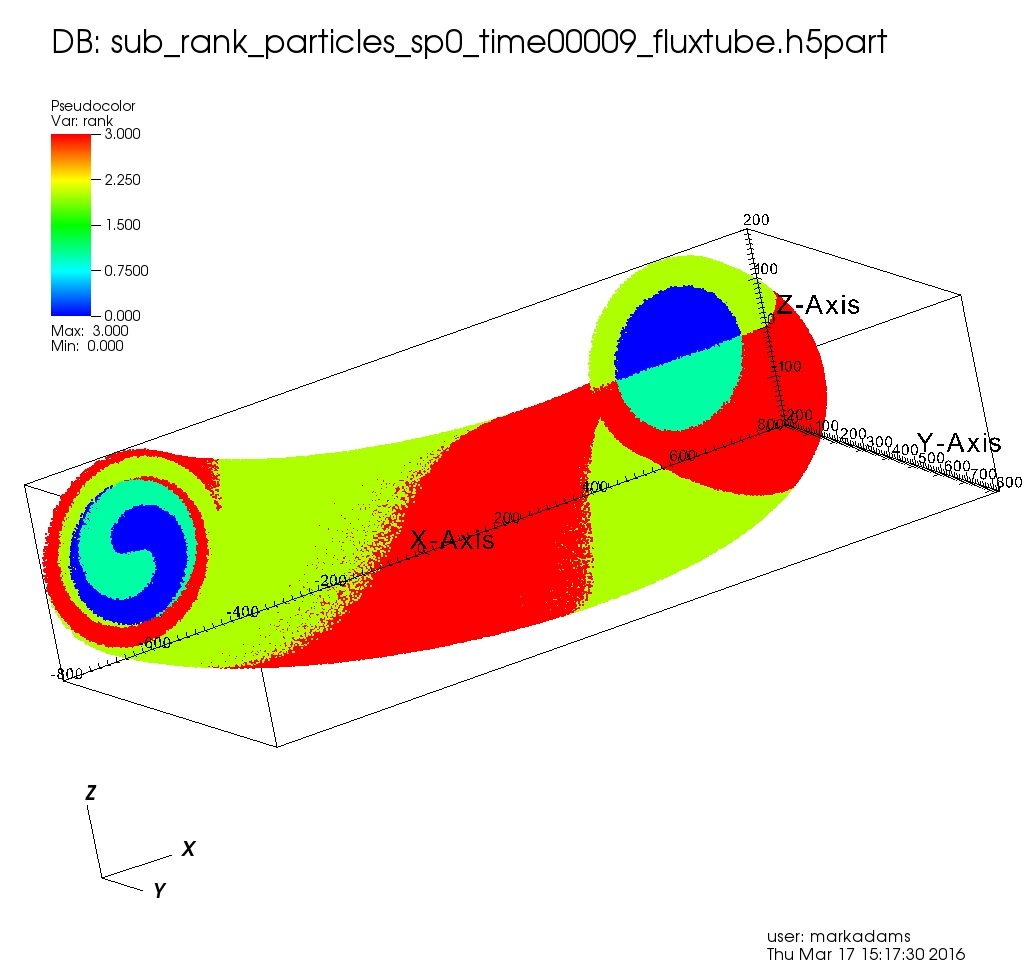
\includegraphics[width=75mm]{half_grid.jpeg} 
    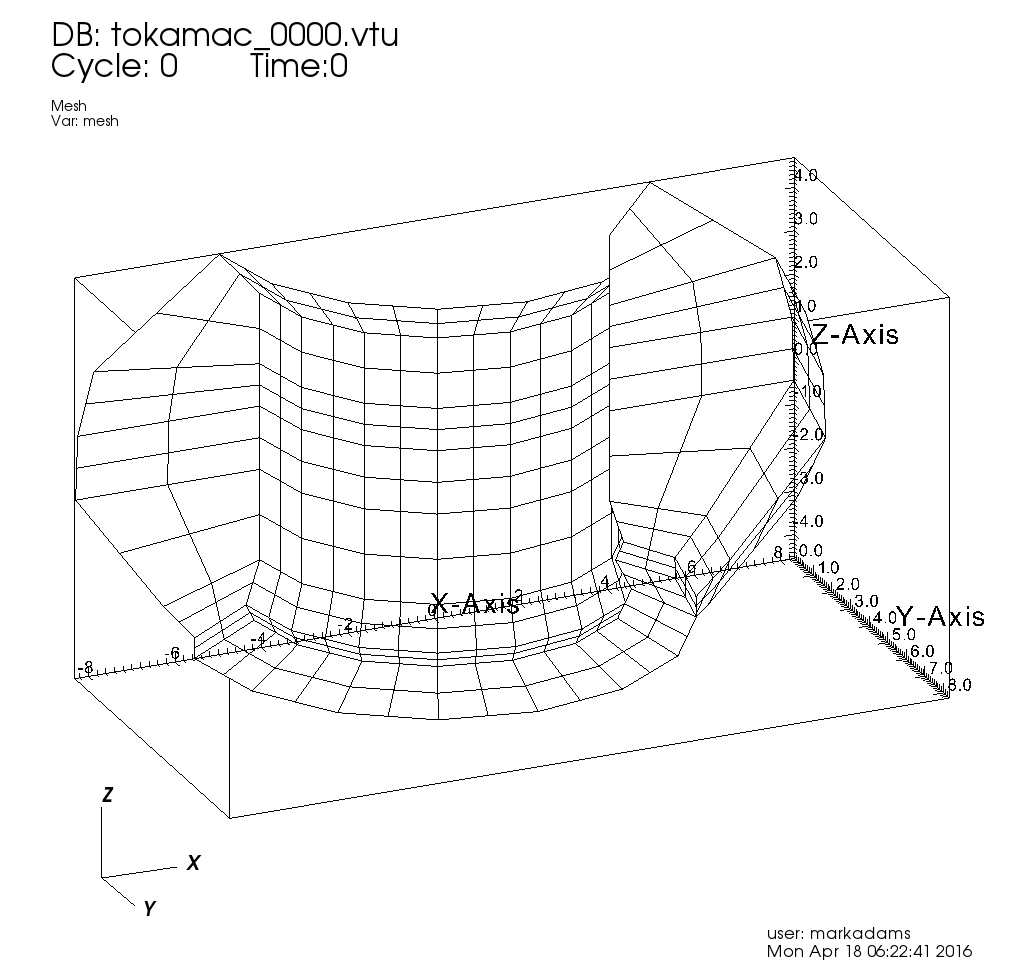
\includegraphics[width=75mm]{half_grid_mesh.jpeg} 
   \caption{Half of  2x2x2 flux tube particle partition of torus (left), corresponding coarse ITER grid solver mesh (right)}
   \label{fig:cross}
\end{figure}
The fuzzy edges of Figure \ref{fig:cross} (left) are due to the finite number of particles, each particle is drawn with the color of the partition to which it belongs.

We currently use trilinear elements, as can be seen in Figure \ref{fig:cross} (right), and intend on using Q2 elements, to resolve the domain more accurately, in the future.
High order elements are attractive because of their high accuracy for smooth solutions should allow for fewer vertices and hence larger ``cells".
Furthermore, because order elements are in effect composed of multiple cells they are still larger in physical space.
Large elements are useful because we use these elements for data locality, larger elements results in larger element particle lists, which are used for vectorization.
Additionally, the solutions of say the Poisson solve in fusion applications, with turbulence, are smooth at the scale of the (known) Larmore radius and, in fact, physicists often smooth the results of low order Poisson solvers to reduce high frequency components.
We plan to move to discontinuous Galerkin (DG) methods in the future because they have attractive mathematical properties, such as having rigorous theory like finite elements and being conservative like finite volume, which would be useful for flux surface averaging projections.
DG results in systems with many degrees of freedom, a common problem of these methods, but fusion PIC solvers are highly over provisioned with processing resources, thus, local work and storage complexity are not critical for these solves.
\bibliographystyle{siamplain}
\bibliography{./bib}


 
\end{document}  